\documentclass[12pt,letterpaper]{article}
\usepackage{graphicx,textcomp}
\usepackage{natbib}
\usepackage{setspace}
\usepackage{fullpage}
\usepackage{color}
\usepackage[reqno]{amsmath}
\usepackage{amsthm}
\usepackage{fancyvrb}
\usepackage{amssymb,enumerate}
\usepackage[all]{xy}
\usepackage{endnotes}
\usepackage{lscape}
\newtheorem{com}{Comment}
\usepackage{float}
\usepackage{hyperref}
\newtheorem{lem} {Lemma}
\newtheorem{prop}{Proposition}
\newtheorem{thm}{Theorem}
\newtheorem{defn}{Definition}
\newtheorem{cor}{Corollary}
\newtheorem{obs}{Observation}
\usepackage[compact]{titlesec}
\usepackage{dcolumn}
\usepackage{tikz}
\usetikzlibrary{arrows}
\usepackage{multirow}
\usepackage{xcolor}
\newcolumntype{.}{D{.}{.}{-1}}
\newcolumntype{d}[1]{D{.}{.}{#1}}
\definecolor{light-gray}{gray}{0.65}
\usepackage{url}
\usepackage{listings}
\usepackage{color}

\definecolor{codegreen}{rgb}{0,0.6,0}
\definecolor{codegray}{rgb}{0.5,0.5,0.5}
\definecolor{codepurple}{rgb}{0.58,0,0.82}
\definecolor{backcolour}{rgb}{0.95,0.95,0.92}

\lstdefinestyle{mystyle}{
	backgroundcolor=\color{backcolour},   
	commentstyle=\color{codegreen},
	keywordstyle=\color{magenta},
	numberstyle=\tiny\color{codegray},
	stringstyle=\color{codepurple},
	basicstyle=\footnotesize,
	breakatwhitespace=false,         
	breaklines=true,                 
	captionpos=b,                    
	keepspaces=true,                 
	numbers=left,                    
	numbersep=5pt,                  
	showspaces=false,                
	showstringspaces=false,
	showtabs=false,                  
	tabsize=2
}
\lstset{style=mystyle}
\newcommand{\Sref}[1]{Section~\ref{#1}}
\newtheorem{hyp}{Hypothesis}

\title{Problem Set 3}
\date{Due: November 12, 2026}
\author{Ethan Kelly Zeh (26359218)}


\begin{document}
	\maketitle
	\section*{Instructions}
	\begin{itemize}
		\item Please show your work! You may lose points by simply writing in the answer. If the problem requires you to execute commands in \texttt{R}, please include the code you used to get your answers. Please also include the \texttt{.R} file that contains your code. If you are not sure if work needs to be shown for a particular problem, please ask.
	\item Your homework should be submitted electronically on GitHub.
	\item This problem set is due before 23:59 on Thursday November 12, 2026. No late assignments will be accepted.

	\end{itemize}

		\vspace{.25cm}
	
\noindent In this problem set, you will run several regressions and create an add variable plot (see the lecture slides) in \texttt{R} using the \texttt{incumbents\_subset.csv} dataset. Include all of your code.

	\vspace{.5cm}
\section*{Question 1}
\vspace{.25cm}
\noindent We are interested in knowing how the difference in campaign spending between incumbent and challenger affects the incumbent's vote share. 
	\begin{enumerate}
		\item Run a regression where the outcome variable is \texttt{voteshare} and the explanatory variable is \texttt{difflog}.	\vspace{.5cm}

		\textbf{Explanation}
		\vspace{.5cm}

		After reading in the data, I first keep only the rows \texttt{voteshare}, \texttt{difflog} and \texttt{presvote}. I then fit the bivariate model:
		\[
		\texttt{voteshare}_i = \beta_0 + \beta_1\,\texttt{difflog}_i + \varepsilon_i
		\]
		with \texttt{lm}. The coefficient on \texttt{difflog} is $0.0417$ ($p < 2\times10^{-16}$) so incumbents who spend more than their challengers by increasing amounts get a larger share of the vote. \texttt{difflog} alone appears to explain about 37\% of the variation in \texttt{voteshare} ($R^2 = 0.367$).
		\vspace{1cm}

		\textbf{Code}
		\lstinputlisting[language=R, firstline=33, lastline=42]{PS03_answersEZ.R}
		\vspace{1cm}
		\textbf{Output}
		\begin{verbatim}
Coefficients:
            Estimate Std. Error t value Pr(>|t|)    
(Intercept) 0.579031   0.002251  257.19   <2e-16 ***
difflog     0.041666   0.000968   43.04   <2e-16 ***

Residual standard error: 0.07867 on 3191 degrees of freedom
Multiple R-squared:  0.3673,	Adjusted R-squared:  0.3671
		\end{verbatim}

		\item Make a scatterplot of the two variables and add the regression line. 	\vspace{.5cm}

		\textbf{Explanation}
		\vspace{.5cm}

		The scatterplot is below. The red line is the fitted line from Question 1(a). There is a clear positive relationship, with the points relatively tightly clustered around the line.
		\vspace{1cm}

		\textbf{Code}
		\lstinputlisting[language=R, firstline=44, lastline=52]{PS03_answersEZ.R}
		\vspace{.5cm}
		\begin{figure}[H]
			\centering
			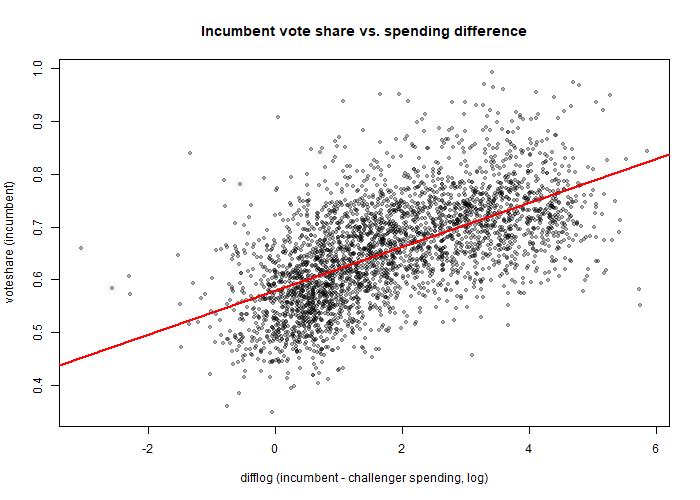
\includegraphics[width=0.8\textwidth]{q1_scatter.png}
		\end{figure}

		\item Save the residuals of the model in a separate object.	\vspace{.5cm}

		\textbf{Explanation}
		\vspace{.5cm}

		The residuals $\hat{\varepsilon}_i = \texttt{voteshare}_i - \widehat{\texttt{voteshare}}_i$ are saved in \texttt{resid\_q1}. They are the part of the incumbent's vote share that is not explained by the spending difference.
		\vspace{1cm}

		\textbf{Code}
		\lstinputlisting[language=R, firstline=54, lastline=55]{PS03_answersEZ.R}

		\item Write the prediction equation.
		\vspace{.5cm}

		Using the coefficients from Question 1(a):
		\[
		\widehat{\texttt{voteshare}}_i = 0.579 + 0.042 \times \texttt{difflog}_i
		\]
		When spending is equal (\texttt{difflog} $= 0$), the predicted incumbent vote share is approx. 57.9\%. Each unit increase in \texttt{difflog} appears to be associated with an increase of approx 4.2 percentage points in the incumbent's vote share.
		\vspace{.5cm}

		\textbf{Code}
		\lstinputlisting[language=R, firstline=57, lastline=58]{PS03_answersEZ.R}
		\vspace{.5cm}
		\textbf{Output}
		\begin{verbatim}
(Intercept)     difflog 
 0.57903071  0.04166632 
		\end{verbatim}
	\end{enumerate}
	
\newpage

\section*{Question 2}
\noindent We are interested in knowing how the difference between incumbent and challenger's spending and the vote share of the presidential candidate of the incumbent's party are related.	\vspace{.25cm}
	\begin{enumerate}
		\item Run a regression where the outcome variable is \texttt{presvote} and the explanatory variable is \texttt{difflog}.	\vspace{.5cm}

		\textbf{Explanation}
		\vspace{.5cm}

		I fit $\texttt{presvote}_i = \beta_0 + \beta_1\,\texttt{difflog}_i + \varepsilon_i$ with \texttt{lm}. The coefficient ofn \texttt{difflog} is $0.0238$ and significant  with ($p < 2\times10^{-16}$), so districts where the incumbent outspends their challenger also appears to give more votes to the presidential candidate of the incumbent's party. However, \texttt{difflog} explains only about 9\% of the variation in \texttt{presvote} ($R^2 = 0.088$).
		\vspace{1cm}

		\textbf{Code}
		\lstinputlisting[language=R, firstline=60, lastline=62]{PS03_answersEZ.R}
		\vspace{1cm}
		\textbf{Output}
		\begin{verbatim}
Coefficients:
            Estimate Std. Error t value Pr(>|t|)    
(Intercept) 0.507583   0.003161  160.60   <2e-16 ***
difflog     0.023837   0.001359   17.54   <2e-16 ***

Residual standard error: 0.1104 on 3191 degrees of freedom
Multiple R-squared:  0.08795,	Adjusted R-squared:  0.08767
		\end{verbatim}

		\item Make a scatterplot of the two variables and add the regression line. 	\vspace{.5cm}

		\textbf{Explanation}
		\vspace{.5cm}

		The fitted line slopes upward, but the points are spread out around it matching the low $R^2$.
		\vspace{1cm}

		\textbf{Code}
		\lstinputlisting[language=R, firstline=64, lastline=72]{PS03_answersEZ.R}
		\vspace{.5cm}
		\begin{figure}[H]
			\centering
			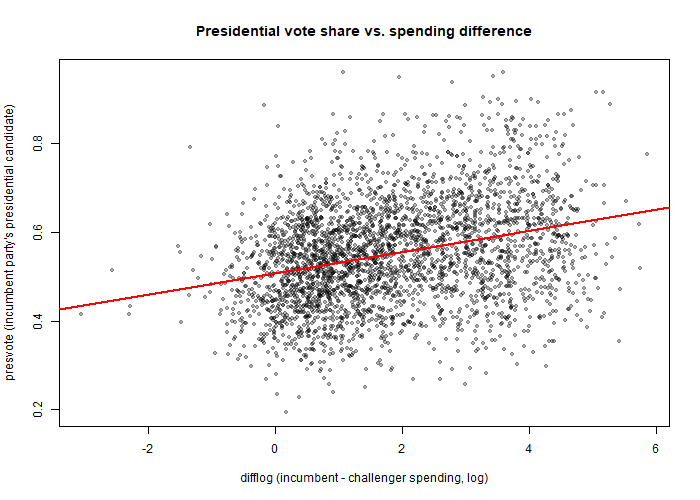
\includegraphics[width=0.8\textwidth]{q2_scatter.png}
		\end{figure}

		\item Save the residuals of the model in a separate object.	\vspace{.5cm}

		\textbf{Explanation}
		\vspace{.5cm}

		The residuals are saved in \texttt{resid\_q2}.
		\vspace{1cm}

		\textbf{Code}
		\lstinputlisting[language=R, firstline=74, lastline=75]{PS03_answersEZ.R}

		\item Write the prediction equation.
		\vspace{.5cm}

		\[
		\widehat{\texttt{presvote}}_i = 0.508 + 0.024 \times \texttt{difflog}_i
		\]
		When spending is equal, the predicted vote share for the incumbent party's presidential candidate is approx. 50.8\%. Each unit increase in \texttt{difflog} is associated with an increase of approx. 2.4 percentage points in \texttt{presvote}.
		\vspace{.5cm}

		\textbf{Code}
		\lstinputlisting[language=R, firstline=77, lastline=78]{PS03_answersEZ.R}
		\vspace{.5cm}
		\textbf{Output}
		\begin{verbatim}
(Intercept)     difflog 
 0.50758333  0.02383723 
		\end{verbatim}
	\end{enumerate}
	
	\newpage	
\section*{Question 3}

\noindent We are interested in knowing how the vote share of the presidential candidate of the incumbent's party is associated with the incumbent's electoral success.
	\vspace{.25cm}
	\begin{enumerate}
		\item Run a regression where the outcome variable is \texttt{voteshare} and the explanatory variable is \texttt{presvote}.
			\vspace{.5cm}

		\textbf{Explanation}
		\vspace{.5cm}

		I fit $\texttt{voteshare}_i = \beta_0 + \beta_1\,\texttt{presvote}_i + \varepsilon_i$ with \texttt{lm}. The coefficient on \texttt{presvote} is $0.388$ ($p < 2\times10^{-16}$): which means that incumbents do better in districts where their party's presidential candidate does better. This appears to explain about 21\% of the variation in \texttt{voteshare} ($R^2 = 0.206$).
		\vspace{1cm}

		\textbf{Code}
		\lstinputlisting[language=R, firstline=80, lastline=82]{PS03_answersEZ.R}
		\vspace{1cm}
		\textbf{Output}
		\begin{verbatim}
Coefficients:
            Estimate Std. Error t value Pr(>|t|)    
(Intercept) 0.441330   0.007599   58.08   <2e-16 ***
presvote    0.388018   0.013493   28.76   <2e-16 ***

Residual standard error: 0.08815 on 3191 degrees of freedom
Multiple R-squared:  0.2058,	Adjusted R-squared:  0.2056
		\end{verbatim}

		\item Make a scatterplot of the two variables and add the regression line. 
			\vspace{.5cm}

		\textbf{Code}
		\lstinputlisting[language=R, firstline=84, lastline=92]{PS03_answersEZ.R}
		\vspace{.5cm}
		\begin{figure}[H]
			\centering
			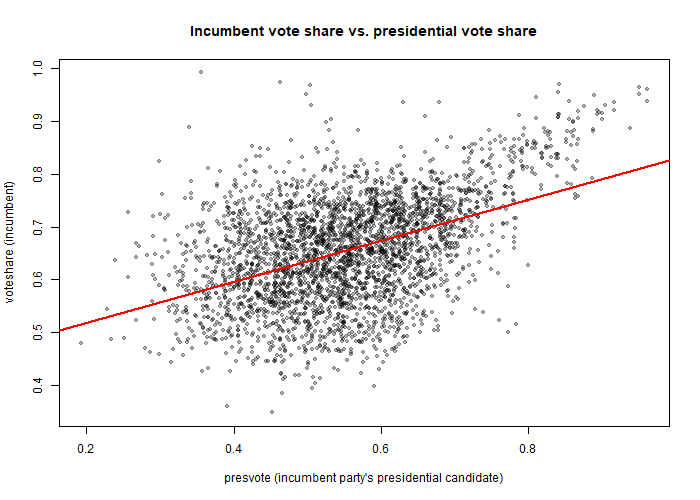
\includegraphics[width=0.8\textwidth]{q3_scatter.png}
		\end{figure}

		\item Write the prediction equation.
		\vspace{.5cm}

		\[
		\widehat{\texttt{voteshare}}_i = 0.441 + 0.388 \times \texttt{presvote}_i
		\]
		A 1 percentage-point increase in the presidential vote share of the incumbent's party is associated with an increase of approx 0.39 percentage points in the incumbents vote share. The intercept (44.1\%) is the predicted vote share if \texttt{presvote} were to be 0, which is not particularly meaningful.
		\vspace{.5cm}

		\textbf{Code}
		\lstinputlisting[language=R, firstline=94, lastline=95]{PS03_answersEZ.R}
		\vspace{.5cm}
		\textbf{Output}
		\begin{verbatim}
(Intercept)    presvote 
  0.4413299   0.3880184 
		\end{verbatim}
	\end{enumerate}
	

\newpage	
\section*{Question 4}
\noindent The residuals from part (a) tell us how much of the variation in \texttt{voteshare} is $not$ explained by the difference in spending between incumbent and challenger. The residuals in part (b) tell us how much of the variation in \texttt{presvote} is $not$ explained by the difference in spending between incumbent and challenger in the district.
	\begin{enumerate}
		\item Run a regression where the outcome variable is the residuals from Question 1 and the explanatory variable is the residuals from Question 2.	\vspace{.5cm}

		\textbf{Explanation}
		\vspace{.5cm}

		Here we regress \texttt{resid\_q1} on \texttt{resid\_q2}. Both residuals no longer have the influence of \texttt{difflog}, so this regression shows the relationship between \texttt{voteshare} and \texttt{presvote} after controlling for the spending difference. The slope(beta) is $0.257$ ($p < 2\times10^{-16}$), smaller than the $0.388$ in Question 3. So, part of the bivariate association in Question 3 appears to have come from the fact that \texttt{difflog} is related to both variables. The intercept is $0$ (expected with OLS residuals).
		\vspace{1cm}

		\textbf{Code}
		\lstinputlisting[language=R, firstline=97, lastline=99]{PS03_answersEZ.R}
		\vspace{1cm}
		\textbf{Output}
		\begin{verbatim}
Coefficients:
             Estimate Std. Error t value Pr(>|t|)    
(Intercept) 3.14e-16   0.001299    0.00        1    
resid_q2    0.256877   0.011762   21.84   <2e-16 ***

Residual standard error: 0.07338 on 3191 degrees of freedom
Multiple R-squared:   0.13,	Adjusted R-squared:  0.1298
		\end{verbatim}

		\item Make a scatterplot of the two residuals and add the regression line. 	\vspace{.5cm}

		\textbf{Explanation}
		\vspace{.5cm}

		The scatterplot for \texttt{presvote}, controlling for \texttt{difflog}. Both axes are centred on zero because they are residuals. The slope of the red line is exactly the coefficient that \texttt{presvote} gets in the multiple regression noted before.
		\vspace{1cm}

		\textbf{Code}
		\lstinputlisting[language=R, firstline=101, lastline=109]{PS03_answersEZ.R}
		\vspace{.5cm}
		\begin{figure}[H]
			\centering
			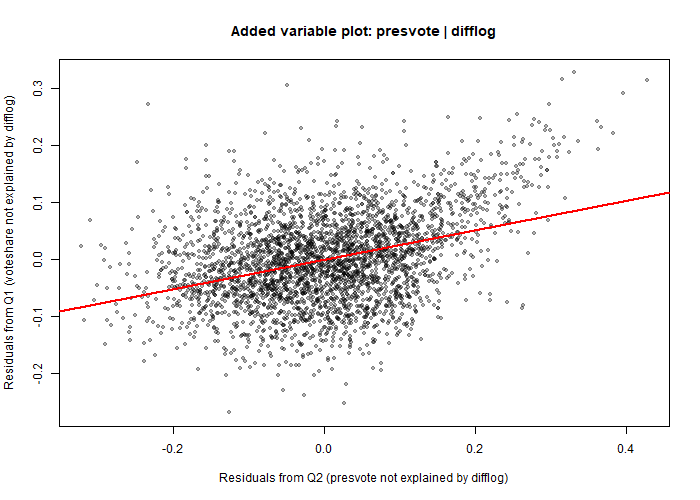
\includegraphics[width=0.8\textwidth]{q4_scatter.png}
		\end{figure}

		\item Write the prediction equation.
		\vspace{.5cm}

		\[
		\widehat{\texttt{resid\_q1}}_i = 0 + 0.257 \times \texttt{resid\_q2}_i
		\]
		A 1 percentage-point increase in \texttt{presvote} spending difference is associated with an increase of approx. 0.26 percentage points in the incumbent's vote share.
		\vspace{.5cm}

		\textbf{Code}
		\lstinputlisting[language=R, firstline=111, lastline=112]{PS03_answersEZ.R}
		\vspace{.5cm}
		\textbf{Output}
		\begin{verbatim}
 (Intercept)     resid_q2 
3.140411e-16 2.568770e-01 
		\end{verbatim}
	\end{enumerate}
	
	\newpage	

\section*{Question 5}
\noindent What if the incumbent's vote share is affected by both the president's popularity and the difference in spending between incumbent and challenger? 
	\begin{enumerate}
		\item Run a regression where the outcome variable is the incumbent's \texttt{voteshare} and the explanatory variables are \texttt{difflog} and \texttt{presvote}.	\vspace{.5cm}

		\textbf{Explanation}
		\vspace{.5cm}

		$\texttt{voteshare}_i = \beta_0 + \beta_1\,\texttt{difflog}_i + \beta_2\,\texttt{presvote}_i + \varepsilon_i$. Both predictors are significant ($p < 2\times10^{-16}$). Together they appear to explain approx 45\% of the variation in \texttt{voteshare} ($R^2 = 0.450$), more than either variable on its own (which were 0.367 and 0.206). The \texttt{difflog} coefficient falls slightly, from $0.0417$ to $0.0355$, after controlling for \texttt{presvote}
		\vspace{1cm}

		\textbf{Code}
		\lstinputlisting[language=R, firstline=114, lastline=116]{PS03_answersEZ.R}
		\vspace{1cm}
		\textbf{Output}
		\begin{verbatim}
Coefficients:
            Estimate Std. Error t value Pr(>|t|)    
(Intercept) 0.448644   0.006330   70.88   <2e-16 ***
difflog     0.035543   0.000946   37.59   <2e-16 ***
presvote    0.256877   0.011764   21.84   <2e-16 ***

Residual standard error: 0.07339 on 3190 degrees of freedom
Multiple R-squared:  0.4496,	Adjusted R-squared:  0.4493
		\end{verbatim}

		\item Write the prediction equation.	\vspace{.5cm}

		\[
		\widehat{\texttt{voteshare}}_i = 0.449 + 0.036 \times \texttt{difflog}_i + 0.257 \times \texttt{presvote}_i
		\]
		When \texttt{presvote} is constant, a one unit increase in \texttt{difflog} is associated with an increase of approx. 3.6 percentage points in the incumbent's vote share. With \texttt{difflog} constant, a 1 percentage-point increase in \texttt{presvote} is associated with an increase of approx. 0.26 percentage points.
		\vspace{.5cm}

		\textbf{Code}
		\lstinputlisting[language=R, firstline=118, lastline=119]{PS03_answersEZ.R}
		\vspace{.5cm}
		\textbf{Output}
		\begin{verbatim}
(Intercept)     difflog    presvote 
 0.44864422  0.03554309  0.25687701 
		\end{verbatim}

		\vspace{1cm}
		\item What is it in this output that is identical to the output in Question 4? Why do you think this is the case?
		\vspace{.5cm}

		The coefficient of \texttt{presvote} ($0.256877$) is identical to the beta of \texttt{resid\_q2} in Question 4 ($0.256877$). The residuals of the two models are also identical (SE is only different due to DF). The standard errors of the slope are therefore almost identical too ($0.011762$ vs.\ $0.011764$).

		\vspace{.5cm}
		In multiple regression the coefficient on \texttt{presvote} measures its effect holding \texttt{difflog} constant, which means it only uses the variation in \texttt{presvote} that is not explained by \texttt{difflog}, which is exactly \texttt{resid\_q2}. Question 4 was done by hand in two steps, and the multiple regression does it all at once, so the answers match. This is also why the name of the plot in Question 4(b) is added variable plot: it shows the relationship that the multiple regression estimates for \texttt{presvote}.
		\vspace{.5cm}

		\textbf{Code}
		\lstinputlisting[language=R, firstline=121, lastline=124]{PS03_answersEZ.R}
		\vspace{.5cm}
		\textbf{Output}
		\begin{verbatim}
Q4 slope: 0.256877 | Q5 presvote coef: 0.256877
		\end{verbatim}
	\end{enumerate}




\end{document}
